\documentclass{article}
\usepackage[utf8]{inputenc}
\usepackage{geometry}
\usepackage{graphicx}
\usepackage{pgfplots}
\usepackage{amsmath}
\usepackage{amssymb}
\usepackage{amsfonts}
\usepackage{mdframed}
\usepackage{amsthm}
\usepackage{physics}
\usepackage{derivative}

\geometry{a4paper, left=2cm, right=2cm, top=1cm, bottom=2cm}

\pgfplotsset{compat=1.18}
\begin{document}

\begin{minipage}{0.7\textwidth}
    \small \textbf{LABORATORIO DE MECÁNICA VECTORIAL}  \\
    \small {Facultad de Ciencias, Universidad Nacional Autónoma de México} \\
    \small {Profesor: Radamés Ricardo Reynoso Manríquez} \\
    \small {Ayudante: Ana Laura Córdova Lara}\\
    \small {Fecha de entrega: 27 de Febrero de 2024} \\
    \small {Nombre completo: Andrés López González} \\
    \small {Tarea número IV}
\end{minipage}
\hfill
\begin{minipage}{0.12\textwidth}
    
\includegraphics[width=\linewidth]{logo_universidad}
\end{minipage}

\section*{Cuestionario III}

PREGUNTA 1. Defina, en términos del cálculo diferencial e integral, a la velocidad. \\\\
\textit{En este contexto, la velocidad se define generalmente como la tasa de cambio de la posición de un objeto respecto al tiempo $\Vec{r}(t)$, pero hay equivalencias para definirla. Se puede expresar de varias formas dependiendo del enfoque como por ejemplo la ya dicha pero en movimiento undimensional, la velocidad como derivada de primer orden de la posición respecto al tiempo $x(t)$, si la posición de un objeto en un espacio unidimensional se denota como $x(t)$, entonces la velocidad $v(t)$ se define como la derivada de $x(t)$ respecto al tiempo $t$, es decir: $v(t) = \frac{dx(t)}{dt}$; por otro lado está la velocidad como derivadas parciales de cada componente en un espacio tridimensional $\Vec{r}(t)$, si la posición de un objeto en el espacio tridimensional se denota como $\Vec{r}(t)=(x(t),y(t),z(t))$, entonces la velocidad $\Vec{v}(t)$ se define como el vector de derivadas parciales de cada componente respecto al tiempo $\mathbf{v}(t) = \frac{d\mathbf{r}(t)}{dt} = \left(\frac{dx(t)}{dt}, \frac{dy(t)}{dt}, \frac{dz(t)}{dt}\right)$; por otro lado también es posible definirla mediante integrales, la velocidad como la integral del vector aceleración $\Vec{a}(t)$. Si la aceleración se denota como $\Vec{a}(t)$, entonces la velocidad $\Vec{V}(t)$ se obtiene mediante la integración de $\Vec{a}(t)$ con respecto al tiempo $\Vec{v}(t) = \int \Vec{a}(t) \, dt$, recordemos del semestre pasado en física contemporánea que cuando tenemos una función multivariable como lo es $\Vec{a}(t)$ y la queremos integrar respecto al tiempo, obtendremos la velocidad, además la constante de integración en este caso (y debería ser siempre) NO debe pasarse por alto, pues esta representa la velocidad inicial $\Vec{v}_0$.}
\\\\

PREGUNTA 2. ¿Bajo qué criterios o premisas se puede hablar de un movimiento rectilíneo uniforme?\\\\
\textit{El movimiento rectilíneo uniforme (MRU) describe el movimiento de un objeto a lo largo de una trayectoria rectilínea con una velocidad constante en el tiempo. Bajo este tipo de movimiento, el objeto no experimenta cambios en su velocidad ni en su dirección a lo largo del tiempo, lo que lo distingue de otros tipos de movimiento más complejos como lo es su hermano mayor el MRUA. Una característica esencial del MRU es que el objeto se desplaza en línea recta, lo que implica que su trayectoria es una línea recta en el espacio. Esta propiedad simplifica el análisis del movimiento, ya que no se requiere considerar cambios en la dirección del objeto, además que utilizando un cambio de base adecuado este movimiento puede ser descrito con una línea recta muy básica; en un MRU, la velocidad del objeto permanece constante en el tiempo. Esto significa que la magnitud de la velocidad, así como su dirección, no experimentan variaciones a lo largo del movimiento. Esta constancia en la velocidad implica que la distancia recorrida por el objeto en intervalos de tiempo iguales es siempre la misma, lo cual es una implicación directa de que la aceleración del objeto es nula, y esto a su vez nos dice que no existe jerk, snap, crackle, pop, entre otras diferenciales de orden mayor igual a dos en la posición respecto al tiempo. La aceleración se define como el cambio en la velocidad en función del tiempo, y al ser constante la velocidad en un MRU su derivada es cero. Otra derivación de la no existencia de aceleraciones es que en un MRU no hay fuerzas externas actuando sobre el objeto que puedan modificar su trayectoria, en palabras simples, no hay fuerzas de fricción, resistencia del aire u otras fuerzas que puedan alterar su velocidad del objeto.}
\\\\

PREGUNTA 3. Haga una lista con las ecuaciones de movimiento para determinar la aceleración en términos de a) posición, y b) velocidad; considerando en ambos casos el parámetro temporal, así como indicar la naturaleza en la diferencia conceptual de la definición de aceleración media, y aceleración instantánea. \\\\
\begin{equation}
v = v_0 + at \quad \Rightarrow \quad a(t) = \frac{v-v_0}{t}
\end{equation}{}
\begin{equation}
x = x_o + v_0t + \frac{at^2}{2} \quad \Rightarrow \quad a(t) = \frac{2(\Delta x - v_0t)}{t^2}
\end{equation}{}
\begin{equation}
\dv[2]{x}{t} = \dv[2]{}{t} \left(x_o + v_0t + \frac{at^2}{2}\right) \quad \Rightarrow \quad a(t) = a
\end{equation}{}
\begin{equation}
v_f^2 = v_0^2 + 2a\Delta x \quad \Rightarrow \quad a(t) = \frac{v_f^2 - v_0^2}{2\Delta x}
\end{equation}
\newpage
\noindent \textit{Usando diferenciales simples.}
\begin{equation}
a(t) = \dv{v}{t} = \dv[2]{x}{t}
\end{equation}
\textit{Usando aproximaciones (aceleración media).}
\begin{equation}
    \Bar{a}(t) = \frac{\Delta v}{\Delta t} = \frac{\Delta x}{\Delta t^2}
\end{equation}
\textit{La diferencia conceptual entre estas dos es que ponemos ver que usamos diferenciales en una y deltas en otro, al usar deltas calculamos la razón de cambio promedio de la función en un intervalo $\Delta t$ no necesariamente pequeño, en cambio en la aceleración instantánea este intervalo es infinitesimal lo que nos proporciona datos precisos (exactos) en ese momento.}\\


PREGUNTA 4. Explique las aplicaciones de los acelerómetros en los dispositivos electrónicos y/o mecánicos. \\\\
\textit{Los acelerómetros brevemente son unos dispositivos usados en el ámbito de la física y la ingeniería, a diferencia de los velocímetros antes analizados, estos, intuitivamente, nos otorgan valores de aceleración en lugar de velocidad; así como con dos velocímetros podemos obtener la aceleración promedio y con varios de estos la tasa de cambio de velocidad, es decir, la segunda derivada de la posición respecto al tiempo (aceleración), con los acerómetros podemos obtener el jerk promedio y con varios de estos la derivada de tercer orden de la posición respecto al tiempo (jerk).}\\

\textit{Uno de los usos más comunes y desapercibidos es en los celulares, estos dispositivos utilizan acelerómetros para detectar cambios en la orientación y el movimiento, lo que permite funciones como la rotación automática de la pantalla y la detección de gestos (como el zigzageo en Motorola para encender la lámpara). Además, los acelerómetros son fundamentales en aplicaciones de realidad aumentada y juegos, donde la detección de movimientos es esencial para la experiencia del usuario.}\\

\textit{Otro campo importante de aplicación de los acelerómetros electrónicos es al igual que los velocímetros en dispositivos de navegación y seguimiento, como sistemas de navegación GPS y dispositivos de seguimiento de actividad física. Los acelerómetros permiten la detección precisa de movimientos, lo que se traduce en mediciones precisas de distancia, velocidad y dirección.}\\

\textit{En el ámbito mecánico, los acelerómetros permiten medir con precisión la aceleración de objetos en movimiento, proporcionando datos fundamentales para entender trayectorias y cambios en la velocidad a lo largo del tiempo, como en el experimento del MRUA donde se simulaba una caída por un plano inclinado y viendo cómo la fuerza normal hacía desplazarse cada vez más rápido el objeto en la componente horizontal. Además, en la biomecánica, estos dispositivos son empleados para estudiar el movimiento humano y animal, posibilitando análisis detallados de la marcha, el rendimiento deportivo y la rehabilitación física. Finalmente otra aplicación interesante es en la detección de terremotos y la monitorización de la actividad sísmica, así como en las pruebas del transporte público (como el metro) en donde se busca que la aceleración sea lo más constante posible para que el jerk sea lo más bajo posible y los pasajeros no perciban esos tirones producto de la tasa de cambio de la aceleración al momento de frenarse o dar curvas tan fuertemente.}
\\\\
\begin{figure} [h]
    \centering
    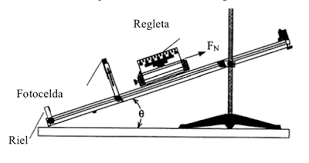
\includegraphics[width=0.45\linewidth]{Regleta.png}
    \caption{MRUA en plano inclinado.}
    \label{fig:enter-label}
\end{figure}\\

\newpage
PREGUNTA 5. Investigue y explique la técnica de la fotografía estroboscópica. \\\\
\textit{La fotografía estroboscópica es una técnica utilizada para capturar imágenes de objetos en movimiento rápido con una clara distinción entre intervalos de tiempo. Esta técnica se basa en el uso de flashes estroboscópicos, que emiten breves pulsos de luz intensa en momentos específicos durante el movimiento del objeto. Estos pulsos de luz con una duración extremadamente corta congelan el movimiento del objeto, permitiendo capturar imágenes nítidas incluso en condiciones de alta velocidad; en nuestro laboratorio los hemos utilizado previamente para obtener datos sobre el MRU y MRUA en condiciones específicas, estos equipos comprenden desde 0 hasta 10,000 flases por minuto (o revoluciones RPM), siendo 7,000 FPM lo que hemos utilizado para asociarlo a los fotogramas que capturaba nuestro obturador del celular.} \\

\textit{Cuando un objeto en movimiento rápido es iluminado por un flash estroboscópico, la luz emitida durante el breve pulso se refleja en el objeto y llega al sensor de la cámara solo por un instante. Debido a la corta duración del pulso de luz, el objeto aparece congelado en la imagen, incluso si se está moviendo a una velocidad considerable; en ocasiones si no se sincroniza perfectamente puede verse ligeramente borrosa la posición del objeto y cuando está completamente desincronizado el fenómeno es análogo a cuando tomamos una foto a un corredor y se ve su "fantasma".} \\

\begin{figure} [h]
    \centering
    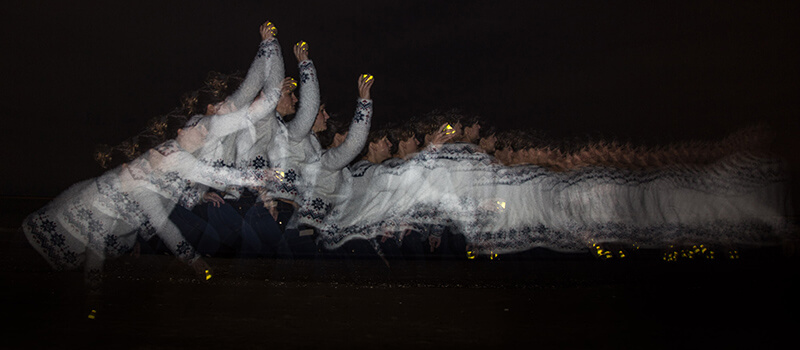
\includegraphics[width=0.5\linewidth]{Estroboscopica.png}
    \caption{Fotografía estroboscópica con excesivamente alta tasa de flashes por minuto}
    \label{fig:enter-label}
\end{figure}

\textit{Esta técnica se utiliza en una amplia gama de aplicaciones, desde la fotografía de alta velocidad en la investigación científica hasta la captura de imágenes creativas en el campo del arte y la fotografía comercial como la adjunta en Figure II. En la investigación científica, la fotografía estroboscópica se utiliza para estudiar el movimiento de objetos en condiciones extremas, como impactos de alta velocidad o fenómenos físicos transitorios.}
\\\\


\end{document}
